\section{Item Interactions}
\label{sec:items}
Items are interactive objects that the player can pick up and use in different situations.

\subsection{Effects for Quests}
In the game, the player will be able to acquire certain items which can trigger new interactions with characters. These items may be given to NPCs in order to start or progress a quest, and some may be used by the player for their own purposes.

\subsubsection{Effects For DISS Battles}
As described in the DISS battle section, the player's \textbf{D.I.S.S.} attributes have an effect on different aspects of the game. The player can use items to buff/debuff these attributes to give them an advantage/disadvantage during a confrontation.

\subsection{Uncollectables}
All interactive objects in the world of \ourgame{} will be implemented using 2D items. Notably, this includes objects such as doors which are actually a part of the 3D environment as can be seen in Figure~\ref{fig:uncollectable drawer}. The difference between these environmental objects and standard items is that they will be flagged as \textbf{uncollectable}. When items are uncollectable, interacting with them will trigger their effects immediately instead of placing them in the player's inventory. For example, interacting with a door would transport the player to another room, and interacting with a container might give the player an item, as shown in Figure~\ref{fig:receive item}.

\begin{figure}[H]
	\centering\begin{subfigure}{.45\textwidth}
		\centering
        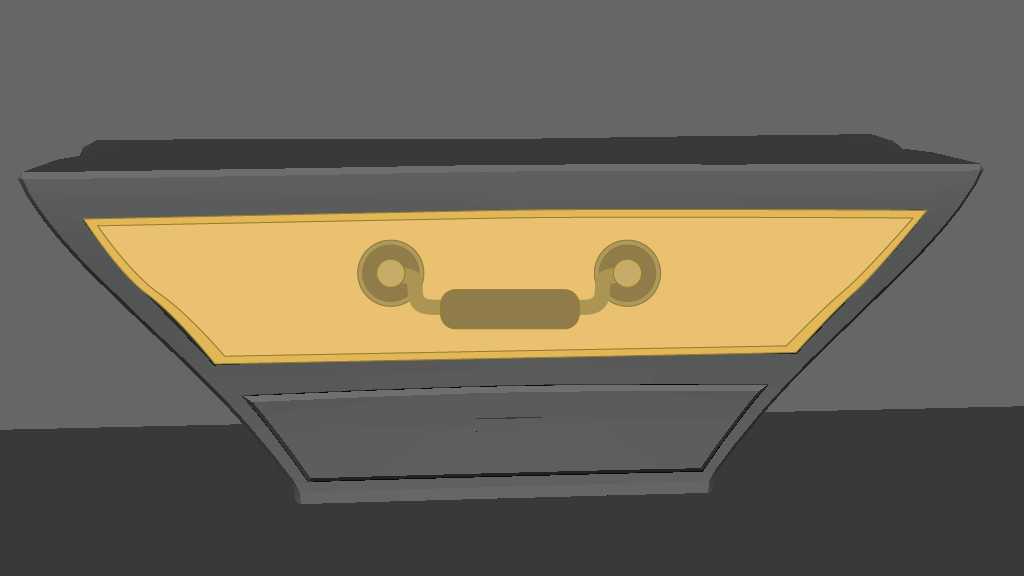
\includegraphics[width=.9\linewidth]{images/container_1}
    	\caption{Interactive but uncollectable drawer item}
    	\label{fig:uncollectable drawer}
    \end{subfigure}
	\begin{subfigure}{.45\textwidth}
		\centering
        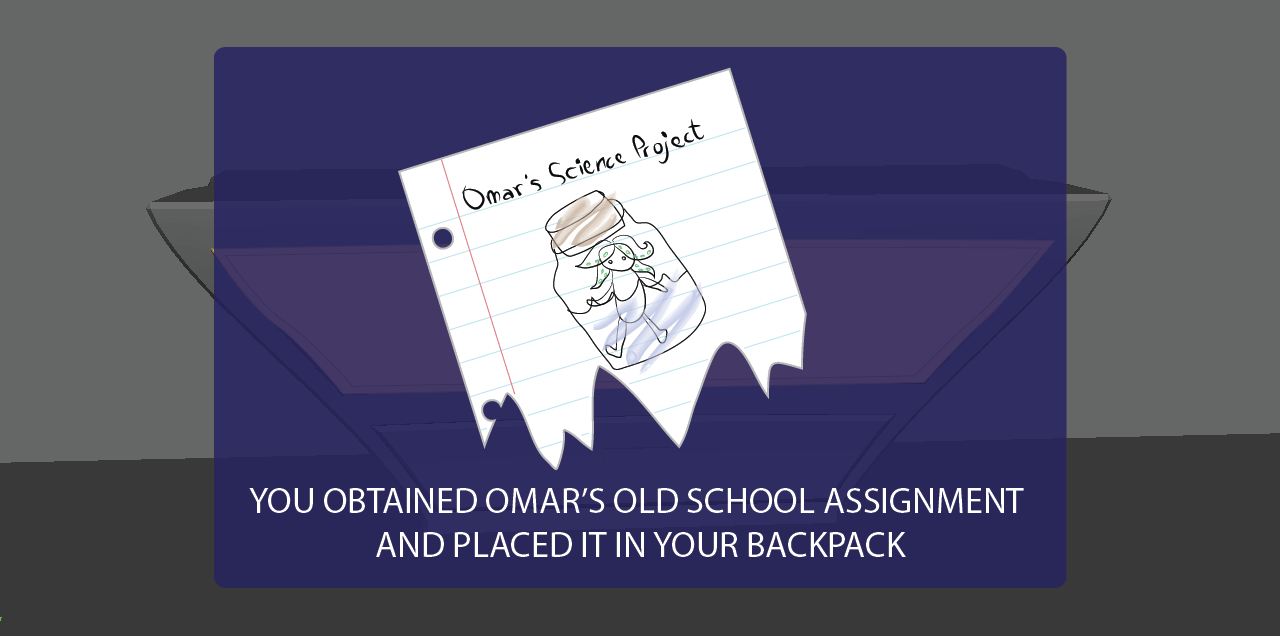
\includegraphics[width=.9\linewidth]{images/container_2}
    	\caption{Receiving an item from an uncollectable container item}
    	\label{fig:receive item}
    \end{subfigure}
    \caption{Example of an uncollectable item interaction}
    \label{fig:uncollectable}
\end{figure}